\subsection{Magic Cube}

\begin{figure}[h]
	\centering
		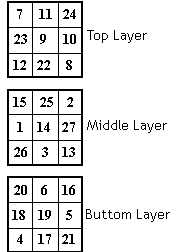
\includegraphics[scale=0.8]{input/pics/presentMagicCube2}
	\caption{\myCaption{This is a magic cube split up into 3 magic squares.}}
	\label{fig:presentMagicCube}
\end{figure}

Both a \msquare{} and a \mcube{} have a magic constant, which can be the sum of each row, column and pillar. However this is where the similarity ends. There are also similarities between the \mcube{} and the \rubik{} which will be elaborated on later.

We have shown how to calculate the magic constant in a \msquare{}.
In a  \mcube{} there is not a big difference in the formula to calculate the magic constant.
\begin{equation}
	M(n)=\frac{n \cdot (n^3+1)}{2}
\end{equation}
As shown in the formula the only difference is the power of $n$ that is changed from 2 to 3.
See appendix \ref{sec:proofOfMagicConstant} for an explanation.

To create a  \mcube{}, there are some parts that need to be explained.
All these basics are shown on figure \ref{fig:cubeparts}.

\begin{figure}[h]
	\centering
		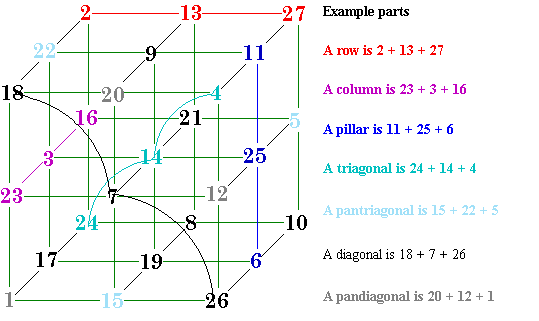
\includegraphics[scale=0.3]{input/pics/cubeparts}
	\caption{\myCaption{This is a Magic Cube where the colors show all of the parts.}}
	\label{fig:cubeparts}
\end{figure}

Because of all these different parts there are a lot of different ways to define  \mcube{}s.
The simplest of them all is a simple  \mcube{}. The only requirements to make such a cube is the following:
\begin{itemize}
	\item All 9 rows, columns and pillars must be equal to the magic constant.
	\item All 4 triagonals must also equal the magic constant.
\end{itemize}

\begin{figure}[h]
	\centering
		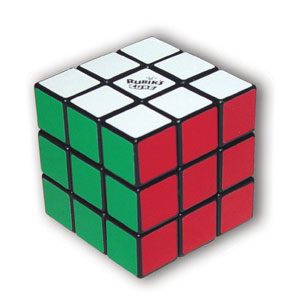
\includegraphics[scale=0.4]{input/pics/rubiksCube}
	\caption{\myCaption{This is a Rubik's Cube.}}
	\label{fig:rubiksCube}
\end{figure}

When looking at the \rubik{} it is easy to see that it looks a lot like the \mcube{}. 
There are two differences. 
The first is that the \mcube{} consists of numbers whereas the \rubik{} has colors, which are different on each \face{}.
The other difference is that the \mcube{} has a number in the center where the \rubik{} center is invisible and out of importancy. This \mcube{} should not be confused with the later presented \mcube{} made by \erno{}.
